\documentclass[black,white]{beamer}

\usepackage{beamerthemesplit}
\usepackage{epstopdf}
\usepackage{graphicx}
\usepackage{subfigure}
\usepackage{hyperref}
\usepackage[utf8]{inputenc}
\usepackage[english]{babel}
\usepackage{listings}
\usepackage{array}
\usepackage{color}
\usepackage{colortbl}

\usefonttheme{professionalfonts}
\usecolortheme{dove}
\useoutertheme{infolines}
\useinnertheme{rectangles}

\setlength{\parindent}{0pt}
\newcommand*\sfb[1]{\textbf{#1}}
\definecolor{red2}{rgb}{.7,0,.39}
\usebackgroundtemplate{
	
\includegraphics[width=\paperwidth,height=\paperheight]{img/bg.png}
}

\begin{document}

\title[LANA for Embedded Devices]{\newline \newline \normalsize{Master Thesis} \newline
				  \huge{\textcolor{red2}{Lightweight Autonomic Network Architecture for Embedded Devices}}}
\author[Daniel Borkmann] {
	\vspace*{-20pt}
	\newline
	Daniel Borkmann	\texttt{<dborkma@tik.ee.ethz.ch>}\\
	\footnotesize{intermediate presentation}
}
\institute[ETH Zurich] {
	Communication Systems Group\\
	ETH Zurich\\\bigskip
	Faculty of Computer Science, Mathematics and Natural Sciences\\
	Leipzig University of Applied Sciences
}
\date[\today]{}

\frame {
	\titlepage
}


\frame {
	\frametitle{\textcolor{red2}{ETH Zurich}}
	\begin{center}
		\hspace*{-40pt}
		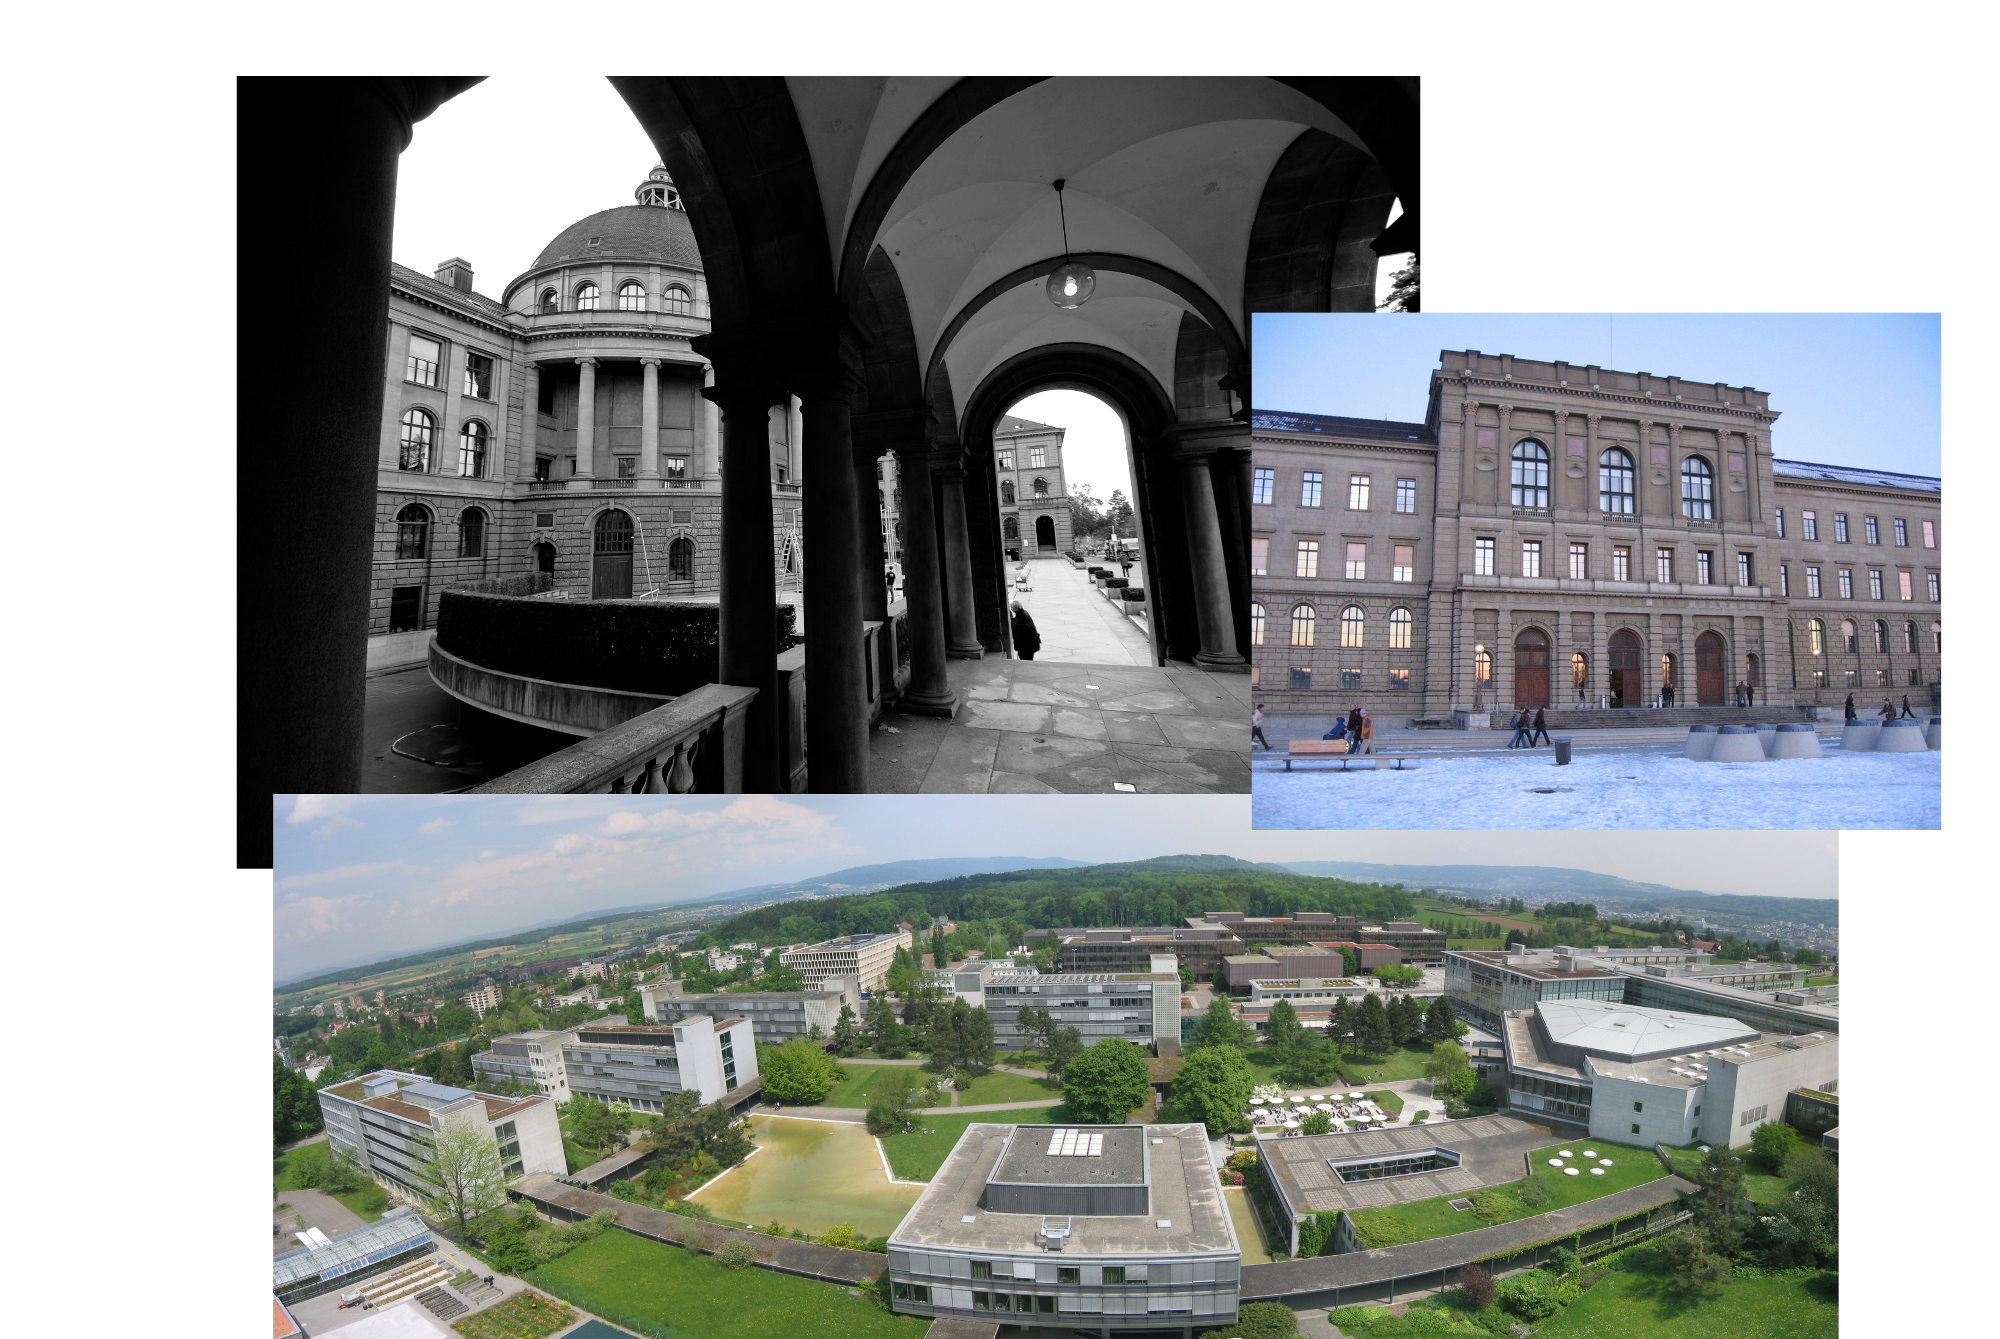
\includegraphics[width=0.9\textwidth]{img/eth.png} \footnotesize{[Src: flickr.com]}
	\end{center}
}

\frame {
	\frametitle{\textcolor{red2}{Communication Systems Group, \newline ETH Zurich}}
	\bigskip
	\begin{itemize}
		\item Communication Systems Group conducts \textbf{research on modeling, design, and implementation of communication systems} [1]:\medskip
		\begin{itemize}
			\item Wireless mobile networks and social networks\medskip
			\item Network measurements and security\medskip
			\item Future Internet architecture and protocols\medskip
		\end{itemize}
		\item \textbf{Thesis advisors:} Ariane Keller, Dr. Wolfgang Mühlbauer\medskip
		\item \textbf{Professor:} Prof. Dr. Bernhard Plattner
	\end{itemize}
}

\frame {
	\frametitle{\textcolor{red2}{Table of Contents}}
	\tableofcontents
}

\section{Introduction}
\subsection{EPiCS Project}
\frame {
	\frametitle{\textcolor{red2}{Introduction}}
	\bigskip
	\bigskip
	\bigskip
	\bigskip
	\bigskip
	\begin{itemize}
		\item Thesis in \textbf{context of the EPiCS} research project [2]\medskip
		\begin{itemize}
			\item Concepts and foundations for self-aware and self-expressive systems\medskip
			\item Hardware/software platform technologies for autonomic compute nodes\medskip
			\item Self-aware network architecture\medskip
		\end{itemize}
		\item For communication purposes, the \textbf{Autonomic Network Architecture (ANA)} [3] will be used
	\end{itemize}

	\vspace*{-20pt}
	\hspace*{+200pt}
	
\includegraphics[width=0.35\textwidth]{img/ana.pdf}
}

\subsection{Basics of ANA}
\frame {
	\frametitle{\textcolor{red2}{Basic idea of ANA}}
	\bigskip
	\bigskip
	\begin{itemize}
		\item \textbf{No "one-size-fits-all" approach} as in classical network architectures\medskip
		\item Network stack is composed by building block processing elements, called \textbf{Functional Blocks (FB)}\medskip
		\item Idea of flexible UNIX Sockets for communication and packet forwarding between Functional Blocks\medskip
		\item Results in a graph of Functional Blocks where the edges represent communication connections\medskip
		\item Packets traverse specific paths of this graph
	\end{itemize}
}

\frame {
	\frametitle{\textcolor{red2}{Basic idea of ANA}}
	\bigskip
	\bigskip
	\bigskip
	\begin{center}
		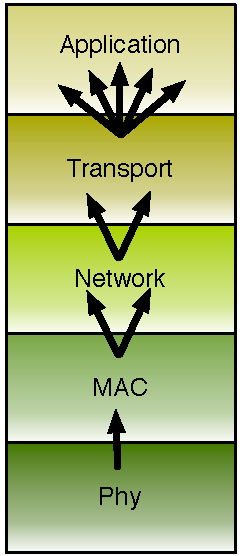
\includegraphics[width=0.20\textwidth]{img/stack_normal.pdf}
		\hspace*{10pt}
		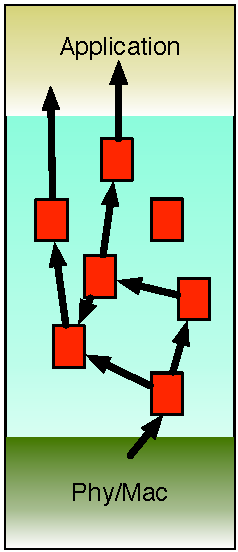
\includegraphics[width=0.20\textwidth]{img/ana_stack.pdf}
	\end{center}
}

\frame {
	\frametitle{\textcolor{red2}{Advantages of this idea}}
	\bigskip
	\begin{itemize}
		\item \textbf{Smaller size of the network stack}\medskip
		\item \textbf{Network stack reconfiguration during runtime}\medskip
		\item Functional Blocks need no a-priori knowledge about their "neighbors"\medskip
		\item Easier to adapt new technologies and protocols\medskip
		\item Application developers do not need to care about underlying addressing schemes, i.e. IPv4 versus IPv6\medskip
		\item \textbf{Not only suited for Internet!}
	\end{itemize}
}

\subsection{Motivation}
\frame {
	\frametitle{\textcolor{red2}{Motivation}}
	\bigskip
	\bigskip
	\begin{itemize}
		\item \textbf{Autonomic Network Architecture important for \newline Embedded Systems [4]}\medskip
		\item Limited resources require network stack adaptions to \newline different networking situations\medskip
		\item Implementation of ANA rather resource-intensive, lightweight \newline redesign is needed\medskip
		\item \textit{Short example:}\medskip
		\begin{itemize}
			\item Currently, packets are being copied between Functional Blocks\medskip
			\item Can be avoided to save CPU processing resources
		\end{itemize}
	\end{itemize}
}

\subsection{Aims of this thesis}
\frame {
	\frametitle{\textcolor{red2}{Aims of this thesis}}
	\bigskip
	\bigskip
	\bigskip
	\begin{itemize}
		\item \textbf{Lightweight redesign and implementation of ANA (LANA)}\medskip
		\item \textit{Requirements:}\medskip
		\begin{itemize}
			\item Needs to outperform the original architecture regarding performance\medskip
			\item Needs to run on embedded Linux devices\medskip
			\item Functional Block adding/removal/swapping during runtime
		\end{itemize}
	\end{itemize}

	\hspace*{+200pt}
	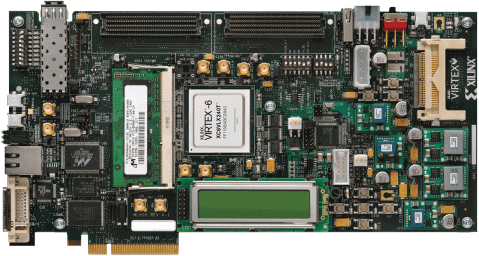
\includegraphics[width=0.35\textwidth]{img/ml605.png}
}

\section{Architectural Changes}
\subsection{Fundamental changes in LANA}
\frame {
	\frametitle{\textcolor{red2}{Fundamental changes in LANA \newline Core Machinery}}
	\bigskip
	\bigskip
	\begin{tabular}{p{0.22\textwidth} p{0.35\textwidth} p{0.35\textwidth}}
	\arrayrulecolor{gray}
		\textbf{Criterion} & \textbf{Current implementation} & \textbf{New implementation}\\[1pt]
		\hline\\[-2.1ex]
		\textit{Message passing between FBs}                       & Memory is copied      & Memory is referenced\\[1pt]
		\hline\\[-2.1ex]
		\textit{API}                         & 3 Layers              & 1 Layer\\[1pt]
		\hline\\[-2.1ex]
		\textit{Threads\footnotemark[1]}     & 1 FB $\hat{=}$ 1 Thread     & "1 CPU $\hat{=}$ 1 Thread"\\[1pt]
		\hline\\[-2.1ex]
		\textit{Centrality\footnotemark[1]}  & Central MINMEX        & Cache-friendly, decentralized\\[1pt]
		\hline\\[-2.1ex]
		\textit{Address space}               & User- and Kernelspace & Kernelspace\\
	\end{tabular}

	\vspace*{-30pt}
	\hspace*{+280pt}
	
\includegraphics[width=0.15\textwidth]{img/tux.png}
	\footnotetext[1]{under the assumption that multiple CPUs are used}
}

\frame {
	\frametitle{\textcolor{red2}{Fundamental changes in LANA \newline Architectural changes}}
	\bigskip
	\bigskip
	\begin{itemize}
		\item New VLink layer for \textbf{virtual networking devices} and \newline \textbf{virtual networks}\medskip
		\item Network stack changes announced via \textbf{Functional Block Notifier}\medskip
		\item Better usage of \textbf{optimized and matured Kernel-APIs}\medskip
		\item Two central userspace tools (\textit{vlink, fbctl}) for administration\medskip
		\item Integration into \textbf{Linux Socket API}
	\end{itemize}

	\vspace*{-30pt}
	\hspace*{+280pt}
	
\includegraphics[width=0.15\textwidth]{img/tux.png}
}

\subsection{Architecture overview}
\frame {
	\frametitle{\textcolor{red2}{Architecture overview}}
	\begin{center}
		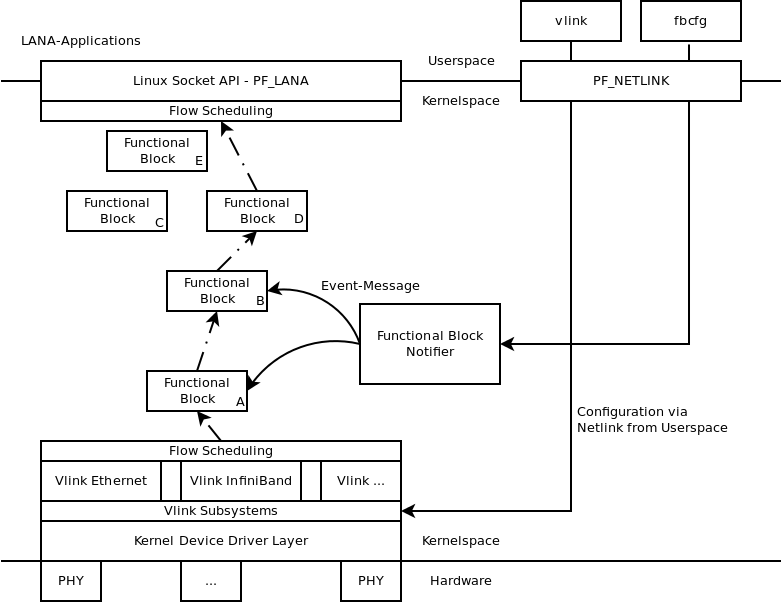
\includegraphics[width=0.73\textwidth]{img/arch.png}
	\end{center}
}

\section{Performance Evaluation and Testing Tools}
\frame {
	\frametitle{\textcolor{red2}{Performance Evaluation and \newline Testing Tools}}
	\bigskip
	\bigskip
	\begin{itemize}
		\item \textbf{Measurement example scenario} (fig. 1)\medskip
		\item Based on the \textbf{netsniff-ng networking toolkit} [5]\medskip
		\item Extended with \textbf{trafgen}, a packet generator\medskip
		\begin{itemize}
			\item Used for performance evaluation, stress-testing, \newline debugging, and the development of LANA\medskip
			\item Uses high-performance Zero-Copy Linux API\medskip
			\item First evaluation shows maximum 422.000 pps \newline (fig. 2, 64 Byte, Gigabit-Ethernet, 2.6 Ghz)\medskip
		\end{itemize}
		\item \textbf{ifpps} used to gather kernel networking statistics\bigskip
	\end{itemize}

	\vspace*{-180pt}
	\hspace*{+245pt}
	\begin{minipage}[h]{0.3\textwidth}
		\begin{flushright}
			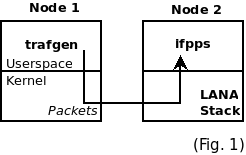
\includegraphics[width=0.9\textwidth]{img/scen.png}\\\medskip
			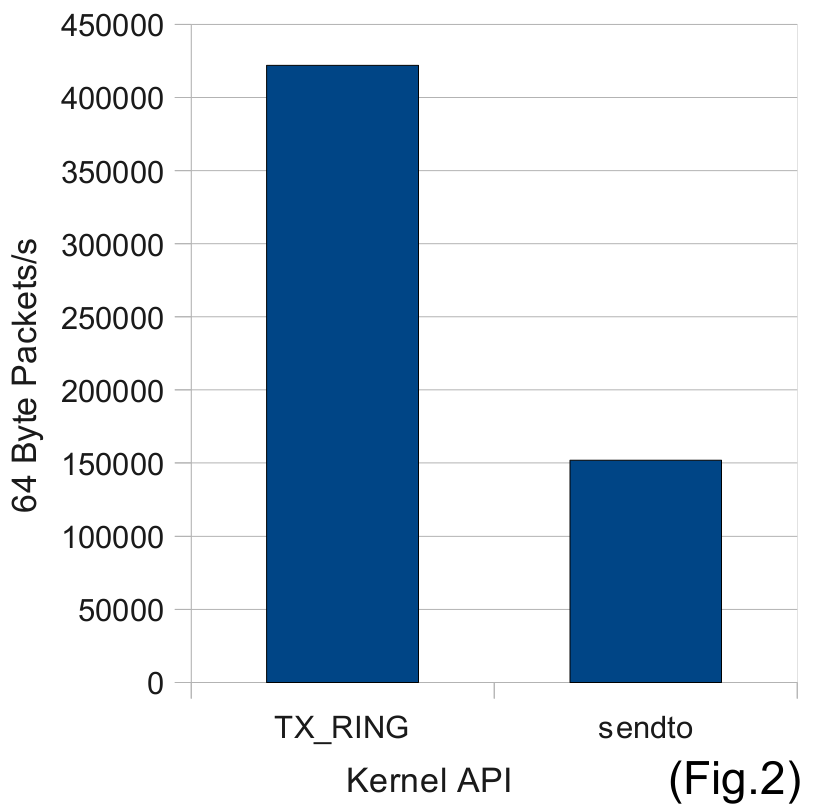
\includegraphics[width=\textwidth]{img/tx.png}
		\end{flushright}
	\end{minipage}
}

\section{Open Questions}
\frame {
	\frametitle{\textcolor{red2}{Open Questions}}
	\bigskip
	\begin{itemize}
		\item What about Userspace Functional Blocks?\medskip
		\item How to find the correct path for network stack traversal?
	\end{itemize}
}

\section{Project Plan}
\frame {
	\frametitle{\textcolor{red2}{Project Plan}}
	\bigskip
	\bigskip
	\bigskip
	\begin{itemize}
		\item Introductory reading, setup of work environment: \textcolor{green}{\textbf{done}}
		\item ANA compilation, test run, written own 'Brick': \textcolor{green}{\textbf{done}}
		\item Architecture design: \textcolor{orange}{\textbf{in progress}}
		\item Implementation of core components: \textcolor{orange}{\textbf{in progress}}
		\item Implementation of 'Functional Blocks': \textcolor{red}{\textbf{to do}}
		\item Testing, debugging: \textcolor{orange}{\textbf{in progress}}
		\item Userspace tools, example applications and manpages: \textcolor{orange}{\textbf{in progress}}
		\item Literature study: \textcolor{orange}{\textbf{in progress}}
		\item Performance evaluation: \textcolor{orange}{\textbf{in progress}}
		\item Final report: \textcolor{red}{\textbf{to do}}
	\end{itemize}
}

\section{Questions}
\frame{
	\frametitle{\textcolor{red2}{Questions}}
	\bigskip
	\bigskip
	\begin{center}
		\Large{Thanks for your attention! Questions?}
	\end{center}
}

\section{Resources}
\frame{
	\frametitle{\textcolor{red2}{Resources}}
	\bigskip
	\bigskip
	\medskip
	\vspace*{-10pt}
	\begin{itemize}
		\item [1]\textbf{CSG, ETH Zurich}, \textcolor{blue}{\url{http://www.csg.ethz.ch/}} (3/2011)\medskip
		\item [2]\textbf{EPiCS project}, \textcolor{blue}{\url{http://www.epics-project.eu/}} (3/2011)\medskip
		\item [3]\textbf{ANA project}, \textcolor{blue}{\url{http://www.ana-project.org/}} (3/2011)\medskip
		\item [4]\textbf{Reconfigurable nodes for future networks}, A. Keller, B. Plattner,
			E. Lübbers, M. Platzner, and C. Plessl in Proc. IEEE Globecom Workshop
			on Network of the Future (FutureNet), pages 372–376. IEEE, Dec. 2010\medskip
		\item [5]\textbf{netsniff-ng}, \textcolor{blue}{\url{http://www.netsniff-ng.org/}} (3/2011)
	\end{itemize}
}

\end{document}

